\chapter{Supplementary Results} % Main appendix title
\label{app:suppresults}
\section{Semantic Embeddings}
\subsection{Visualization of Semantic Spaces with TensorFlow Projector}
\label{appsubsec:projectorvisu}

The French \code{SIM} space's first four PCs encodes POS information. Thus the 3D PCA presentation of \code{SIM} is three axes parallel to the visualization axes (Figure \ref{fig:freSIMmarcher}). 
\begin{table}
    \centering
    \begin{tabularx}{\textwidth}{*{4}{P{.23\textwidth}}}
    \mc{4}{l}{\tabhead{French Semantic Embeddings}} \\
    \mc{4}{l}{\tabhead{Target word:} professeur\_n} \\
    \toprule
    \code{SIM} & \code{SIG}& \code{ASN} & \code{MIX} \\
    \toprule
    pédagogue\_n & pédagogue\_n & fondateur\_n & naissance\_n\\
éducateur\_n & éducateur\_n & psychose\_n & psychose\_n\\
instituteur\_n & instructeur\_n & éducation\_n & éducation\_n\\
instructeur\_n & instituteur\_n & serveur\_n & secrétaire\_n\\
arbitre\_n & arbitre\_n & secrétaire\_n & logique\_a\\
lecteur\_n & adjudant\_n & défenseur\_n & fondateur\_n\\
enseignant\_n & passe\_n & imitation\_n & chronique\_a\\
passe-partout\_n & passe-partout\_n & vicaire\_n & imitation\_n\\
passepartout\_n & lecteur\_n & sensation\_n & sensation\_n\\
passe\_n & enseignant\_n & protecteur\_n & honneur\_n\\
adjudant\_n & abonné\_n & protectionnisme\_n & traumatisme\_n\\
aide\_de\_camp\_n & maestro\_n & volontaire\_n & vicaire\_n\\
maître\_n & spécialiste\_n & fonctionnaire\_n & facilité\_n\\
maestro\_n & châtelain\_n & naissance\_n & serveur\_n\\
capitaine\_de\\ \_vaisseau\_n & capitaine\_n & photographie\_n & proposition\_n\\
maître\_d'hôtel\_n & commandant\_n & producteur\_n & disparition\_n\\
commandant\_n & propriétaire\_n & évidence\_n & moteur\_n\\
capitaine\_n & professionnel\_n & honneur\_n & sagesse\_n\\
spécialiste\_n & leader\_n & croisade\_n & croisade\_n\\
commandement\_n & contributeur\_n & missionnaire\_n & évidence\_n\\
abonné\_n & possesseur\_n & moteur\_n & quantité\_n\\
overlord\_n & savant\_n & pluralisme\_n & défaillance\_n\\
châtelain\_n & commandement\_n & sagesse\_n & édition\_n\\
précepte\_n & acquéreur\_n & coexistence\_n & défenseur\_n\\
fondateur\_n & acheteur\_n & objectif\_a & volontaire\_n\\
débutant\_n & participant\_n & facilité\_n & protecteur\_n\\
tyro\_n & officiel\_n & disparition\_n & pluralisme\_n\\
\bottomrule
    \end{tabularx}
    \caption[Exemplar Neighborhoods in French Semantic Embeddings]{}
    \label{tab:freNeighbour}
    \end{table}


\begin{figure}
    \centering
    \begin{minipage}[t]{.5\textwidth}
        \centering
        \makebox[.5\linewidth]{
        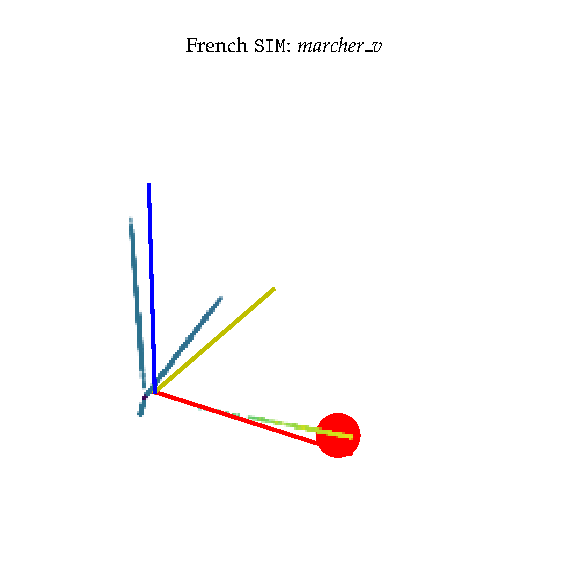
\includegraphics[scale=1]{Figures/FreSIMPCAformarcher_v.pdf}
        }
        \caption[French \code{SIM} Space Visualization]{Due to the nature of WOLF, 
        \code{SIM}'s first PCs denotes POS category. Light colors indicate the proximity of the represented words with \emph{marcher\_v}.}
        \label{fig:freSIMmarcher}
    \end{minipage}%
    \begin{minipage}[t]{.5\textwidth}
        \centering
        \makebox[.5\linewidth]{
        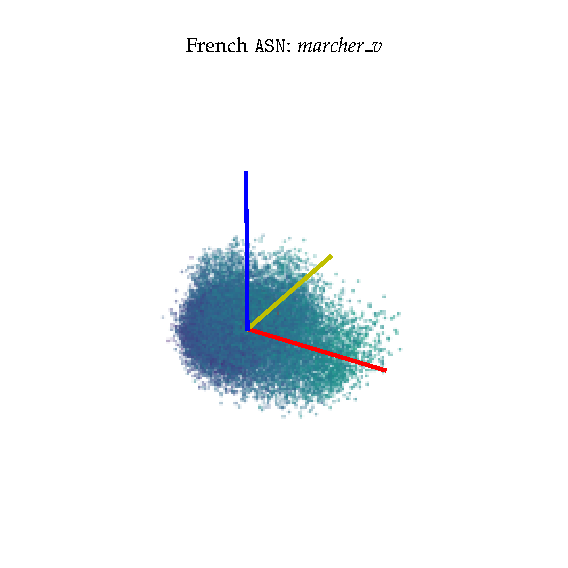
\includegraphics[scale=1]{Figures/FreASNPCAformarcher_v.pdf}
        }
        \caption[French \code{ASN} Space Visualization]{\code{ASN}'s variance are more homogeneously distributed over PCs.}
        \label{fig:freASNmarcher}
    \end{minipage}
\end{figure}


\begin{figure}
    \centering
    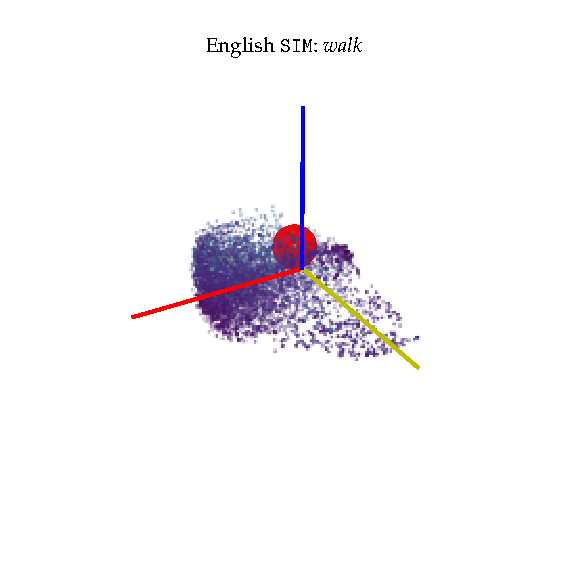
\includegraphics[scale=1]{Figures/EngSIMPCAforwalk.pdf}
    \caption[English \code{SIM} Space Visualization]{English's \code{SIM} however seems not to be macroscopically influenced by POS information.}
    \label{fig:engSIMwalk}
\end{figure}

\subsection{Semantic Ranking Task Results}
\label{appsubsec:wnembeddingtests}
\begin{table}
 \centering
 \begin{ThreePartTable} 
\begin{tabularx}{\textwidth}{p{3cm} *{2}{p{.5cm}} *{2}{p{1.7cm}} *{4}{L}} 
\multicolumn{8}{l}{\tabhead{English \code{WordNetEmbedding} Iterations}} \\
 \toprule
 \mr{2}{=}{\tabhead{Relations}} & \mr{2}{=}{\rotatebox[origin=c]{90}{\tabhead{Lexicon}}} & \mr{2}{=}{\rotatebox[origin=c]{90}{\tabhead{Dim.}}} & \mr{2}{=}{\tabhead{Metric}}  & \mc{3}{l}{\tabhead{\emph{Similarity}}} & \tabhead{\emph{Association}} \\
 \cmidrule{5-7}
 & & & & \small{\textbf{SIMLEX-999}} & \small{\textbf{WS353-SIM}} & \small{\textbf{RG1965}} & \small{\textbf{WS353-ASN}} \\
 \toprule
 \mr{4}{=}{\textbf{S}ynonymy} &\mr{2}{=}{15k}  & \mr{12}{=}{850} & Pearson & .2256 & .2679 & .3627 & .123 \\
 & & & Spearman & .2001 & .2003 & .3403 & .0971 \\
\cmidrule{2-2} \cmidrule{4-8}
  & \mr{2}{=}{60k} &  & Pearson & .234 & .2112 & .3394 & .1449 \\
 & & & Spearman & .1747 & .1895 & .2629 & .1129 \\
 \cmidrule{1-2} \cmidrule{4-8}
 \mr{2}{=}{S+Antonymy} & \mr{6}{=}{15k} &  & Pearson & .1534 & .2743 & .373 & .0969 \\
 & & & Spearman & .1255 & .1922 & .3302 & .0817 \\
 \cmidrule{1-1} \cmidrule{4-8}
 \mr{2}{=}{S+\textbf{H}yp\textbf{e}r/\textbf{H}yp\textbf{o}nymy} &  &  & Pearson & .3904 & .4825 & .6187 & .0373 \\
 & & & Spearman & .4018 & .3856 & .5145 & .0259 \\
 \cmidrule{1-1} \cmidrule{4-8}
 \mr{6}{=}{SHeHo+ adj.participle\_of\_verb+ adj.similar+ adv.derive\_from\_adj} &  &  & Pearson & .5079 & .5333 & .6784 & .0525 \\
 & & & Spearman & .4986 & .4214 & .576 & .0272 \\
 \cmidrule{2-2} \cmidrule{4-8}
  & \mr{2}{=}{60k} &  & Pearson & .5268 & .5483 & .6991 & .1092 \\
 & & & Spearman & .5152 & .4757 & .5501 & .0515 \\
 \cmidrule{2-8}
  & \mr{2}{=}{15k\tnote{0}}  & \mr{2}{=}{511} & Pearson & .506 & & & .0279 \\
 & & & Spearman & .4989 & & & .0193 \\
 \cmidrule{2-8} 

&  & \mc{2}{r}{Out Of Vocabulary} & .002 & .02 & 0 & .012 \\
\midrule
\mr{4}{=}{All\tnote{1}} & \mr{2}{=}{13k\tnote{2}} & \mr{8}{=}{850} & Pearson & .5 & .65 & .65 & .32 \\
 & & & Spearman & .52 & .67 & .75 & .33 \\
\cmidrule{2-2} \cmidrule{4-8}
 & \mr{2}{=}{60k\tnote{3}} & & Pearson & .5 & .51 & .56 & .31 \\
 & & & Spearman & .51 & .58 & .72 & .3 \\
\cmidrule{1-2} \cmidrule{4-8}
 \mr{3}{=}{Synonym Database\tnote{4}} & \mr{2}{=}{60k\tnote{5}} &  & Pearson & .6814 & .5819 & .8155 & .317 \\
 & & & Spearman & .6566 & .4677 & .7032 & .3153 \\
 \cmidrule{2-8}
 & & \mc{2}{r}{Out Of Vocabulary} & .066 & .227 & .077 & .19 \\
\bottomrule
\end{tabularx}
\begin{tablenotes}
    \footnotesize
    \item[0] Version reported in Table \ref{tab:engdecorrelationscores}.
    \item[1] Data reported by \textcite{saediWordNetEmbeddings2018}.
    \item[2] Cue words selected from psycholinguistic experiment datasets.
    \item[3] Words selected randomly. On the contrary, our implementation selects the top 60k most frequent words in \code{WordNet}. 
    \item[4] Synonym database is created by thesauri fusion and symmetrization. Data provided by \textcite{plouxModelMatchingSemantic2003}.
    \item[5] The synonym database contains multi-word phrases, whereas task benchmarks only test for single-word pairs. The actual lexicon size of the database is 36718.
\end{tablenotes}
\end{ThreePartTable}
\caption[English \code{WordNetEmbedding} Iterations]{Placeholder \label{apptab:engWordNetIteration}}
\end{table}

% \begin{table}
%     \centering
%     \begin{ThreePartTable} 
%    \begin{tabularx}{\textwidth}{p{3cm} *{3}{R} *{4}{L}} 
% \multicolumn{8}{l}{\tabhead{English Dissociation}} \\
%  \toprule
%  \mr{2}{=}{Common Crawl} & 2.2M, cased & 300 & Pearson & .3946 & .6573 & .6812 & .6091 \\
%  & & & Spearman & .3752 & .6298 & .6577 & .5709 \\
%  & & & OOV & .1 & 0 & 0 & 0 \\
%  \mr{2}{=}{CommonCraw - 01-23 Sim} & 8157 & 300 & Pearson & .1953 & .5854 & .5547 & .5633 \\
%  & & & Spearman & .2133 & .5719 & .5641 & .5918 \\
%  & & & OOV & & & & \\
%  \bottomrule
% \end{tabularx}
% \end{ThreePartTable}
% \caption[English Semantic Space Dissociation]{Placeholder \label{apptab:engDissociation}}
% \end{table}

\subsection{Vocabulary Coverage by POS}
\begin{table}
    \centering
    \begin{ThreePartTable}  
    \begin{tabularx}{\textwidth}{L *{10}{R}}
    \multicolumn{11}{l}{\tabhead{The Little Prince Vocabulary Coverage}} \\
    \toprule
    &  & \multicolumn{9}{l}{\tabhead{\# Instances in fMRI Recording Session}} \\
    \toprule
    &  & \tabhead{R1} & \tabhead{R2} & \tabhead{R3}& \tabhead{R4}& \tabhead{R5}& \tabhead{R6}& \tabhead{R7}& \tabhead{R8}& \tabhead{R9}\\
    \toprule
    \multicolumn{11}{l}{\tabhead{Nouns}} \\
    \toprule
    \mr{2}{*}{Story} & \textbf{T} &  269 & 286 & 306 & 242 & 284 & 355 & 281 & 265 & 246 \\
     & \textbf{V} & 142 & 140 & 152 & 107 & 108 & 147 & 109 & 135 & 121 \\
    \midrule
    \mr{4}{*}{\parbox{0.8cm}{\code{SIM} 56665}} & TM & 17 & 3 & 7 & 5 & 14 & 14 & 11 & 11 & 16 \\
     & \% & 6.32 & 1.05 & 2.29 & 2.07 & 4.93 & 3.94 & 3.91 & 4.15 & 6.50 \\
     & VM & 10 & 3 & 6 & 3 & 3 & 8 & 6 & 7 & 7 \\
     & \% & 7.04 & 2.14 & 3.95 & 2.80 & 2.78 & 5.44 & 5.50 & 5.19 & 5.79 \\
    \midrule
    \mr{4}{*}{\parbox{0.8cm}{\code{ASN} /\code{MIX} /\code{SIG} 24519}} & TM & 20 & 9 & 8 & 10 & 22 & 16 & 11 & 13 & 17 \\
     & \% & 7.43 & 3.15 & 2.61 & 4.13 & 7.75 & 4.51 & 3.91 & 4.91 & 6.91 \\
     & VM & 12 & 5 & 7 & 4 & 7 & 10 & 6 & 8 & 8 \\
     & \% & 8.45 & 3.57 & 4.61 & 3.74 & 6.48 & 6.80 & 5.50 & 5.93 & 6.61 \\
     \toprule
    \multicolumn{11}{l}{\tabhead{Verbs}} \\
    \toprule
    \mr{2}{*}{Story} & \textbf{T} & 227 & 274 & 313 & 306 & 258 & 296 & 331 & 278 & 335 \\
     & \textbf{V} & 104 & 109 & 142 & 119 & 84 & 113 & 99 & 110 & 118 \\
    \midrule
    \mr{4}{*}{\parbox{0.8cm}{\code{SIM} 56665}} & TM & 9 & 15 & 14 & 15 & 10 & 4 & 7 & 12 & 7 \\
     & \% & 3.96 & 5.47 & 4.47 & 4.90 & 3.88 & 1.35 & 2.11 & 4.32 & 2.09 \\
     & VM & 7 & 7 & 9 & 11 & 9 & 4 & 5 & 8 & 6 \\
     & \% & 6.73 & 6.42 & 6.34 & 9.24 & 10.71 & 3.54 & 5.05 & 7.27 & 5.08 \\
    \midrule
    \mr{4}{*}{\parbox{0.8cm}{\code{ASN} /\code{MIX} /\code{SIG} 24519}} & TM & 9 & 19 & 15 & 17 & 10 & 8 & 9 & 12 & 14 \\
     & \% & 3.96 & 6.93 & 4.79 & 5.56 & 3.88 & 2.70 & 2.72 & 4.32 & 4.18 \\
     & VM & 7 & 10 & 10 & 13 & 9 & 7 & 6 & 8 & 10 \\
     & \% & 6.73 & 9.17 & 7.04 & 10.92 & 10.71 & 6.19 & 6.06 & 7.27 & 8.47 \\
     \toprule
     \multicolumn{11}{l}{\tabhead{Adjectives \& Adverbs}} \\
     \toprule
     \mr{2}{*}{Story} & \textbf{T} & 229 & 252 & 241 & 214 & 190 & 251 & 207 & 169 & 221 \\
     & \textbf{V} & 102 & 111 & 117 & 103 & 100 & 107 & 94 & 83 & 104 \\
     \midrule
     \mr{4}{*}{\parbox{0.8cm}{\code{SIM} 56665}} & TM & 10 & 12 & 11 & 7 & 6 & 15 & 6 & 7 & 4 \\
      & \% & 4.37 & 4.76 & 4.56 & 3.27 & 3.16 & 5.98 & 2.90 & 4.14 & 1.81 \\
     & VM & 9 & 6 & 7 & 6 & 4 & 7 & 5 & 4 & 3 \\
     & \% & 8.82 & 5.41 & 5.98 & 5.83 & 4.00 & 6.54 & 5.32 & 4.82 & 2.88 \\
     \midrule
     \mr{4}{*}{\parbox{0.8cm}{\code{ASN} /\code{MIX} /\code{SIG} 24519}} & TM & 19 & 19 & 15 & 10 & 16 & 36 & 15 & 12 & 10 \\
      & \% & 8.30 & 7.54 & 6.22 & 4.67 & 8.42 & 14.34 & 7.25 & 7.10 & 4.52 \\
      & VM & 11 & 11 & 9 & 8 & 10 & 15 & 8 & 6 & 7 \\
      & \% & 10.78 & 9.91 & 7.69 & 7.77 & 10.00 & 14.02 & 8.51 & 7.23 & 6.73 \\
    \bottomrule
    \end{tabularx}
    \end{ThreePartTable}
    \caption[The Little Prince Vocabulary Coverage by POS]{\textbf{T}: Token, \textbf{V}: Lexicon Unit, M: Miss\label{apptab:lppcoverage}}
    \end{table}


\subsection{Corpus-Targeted Semantic Feature Selection}
[TODO still necessary?]


\section{Non-nested Model Comparison}
\label{appsubsec:nonnestedcompres}

\subsubsection{Use \code{SIM} to Predict \code{ASN}}
[TODO, insert heat-map of coefficients]
Each of the 203 columns in the \code{ASN} class design matrix (including non-semantic features) are predicted by 103 columns of the \code{SIM} class design matrix. We averaged the \code{r2} score of each column model across 9 cross-validation runs. The histogram of the scores are plotted in Figure \ref{fig:SIMASNDist}, informative model scores are presented in Table \ref{tab:SIMASNScores}. As our design-matrices are orthonormalized, columns sitting at larger indexes have a dependency on smaller-indexed columns. The first columns being bell predicted start at index 12 (to 14). Other columns are scattered up to index 47. We can therefore conclude that the predictability found are purely due to numerical coincidences.

\begin{figure}
    \centering
    \begin{minipage}[t]{.5\textwidth}
        \centering
        \makebox[.5\linewidth]{
            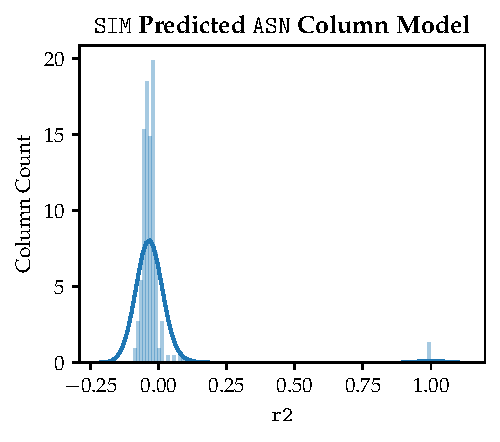
\includegraphics[scale=.8]{Figures/SIMASNDist.pdf}
            }
            \caption[\texttt{SIM} Predicted \texttt{ASN} Column Model]{3 columns are perfectly predicted as they are non-semantic features that are shared by the design matrices. For the rest most of the column-models are worse than arbitrary models.} 
            \label{fig:SIMASNDist}
    \end{minipage}%
    \begin{minipage}[t]{.5\textwidth}
        \centering
        \makebox[.5\linewidth]{
            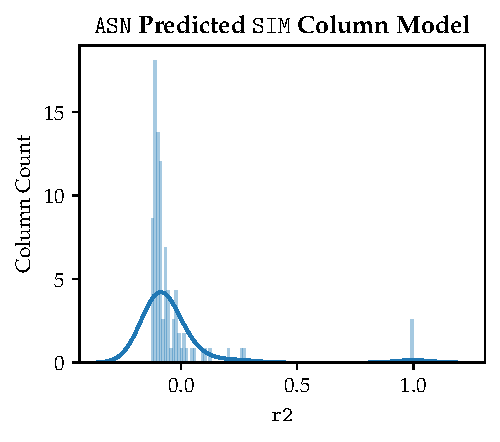
\includegraphics[scale=.8]{Figures/ASNSIMDist.pdf}
            }
            \caption[\texttt{ASN} Predicted \texttt{SIM} Column Model]{Most of the column-models are worse than arbitrary models. More columns in \code{SIM} are better predicted with \code{ASN} design matrices.} 
            \label{fig:ASNSIMDist}
    \end{minipage}
\end{figure}


\begin{table}
    \centering
    \begin{ThreePartTable}
    \begin{tabularx}{\textwidth}{p{1.7cm} *{11}{L}}
    \mc{12}{l}{\tabhead{\texttt{SIM} Predicted \texttt{ASN} Column Model Performances}} \\
    \toprule
    \tabhead{Col Index} & 22 & 20 & 14 & 37 & 47 & 18 & 27 & 26 & 13 & 12 & 30 \\  
    \tabhead{\code{r2}} & .0891 & .0834 & .0548 & .0346 & .0164 & .0152 & .0122 & .0113 & .0112 & .0075 & .0004 \\  
    \tabhead{\code{r}} & .2984 & .2887 & .2340 & .1861 & .1279 & .1233 & .1104 & .1064 & .1058 & .0867 & .0203 \\
    \bottomrule
    \end{tabularx}
    \end{ThreePartTable}
    \caption[\texttt{SIM} Predicted \texttt{ASN} Column Model Performances]{Index starts at 0, \code{ASN} group features starts from 3.  Among the 14 informative models (\code{r2} > 0), 3 are non-semantic features (not listed above). Pearson's \code{r} are converted from \code{r2}. \label{tab:SIMASNScores}}
\end{table}

\begin{table}
    \centering
    \begin{ThreePartTable}
    \begin{tabularx}{\textwidth}{p{1.7cm} *{11}{L}}
    \mc{12}{l}{\tabhead{\texttt{ASN} Predicted \texttt{SIM} Column Model Performances}} \\
    \toprule
    \tabhead{Col Index} & 6 & 3 & 5 & 11 & 4 & 7 & 75 & 18 & 42 & 25 & 47 \\  
    \tabhead{\code{r2}} & .2761 & .2646 & .2041 & .1256 & .1032 & .0971 & .0529 & .0485 & .0192 & .0158 & .0107 \\  
    \tabhead{\code{r}} & .5254 & .5144 & .4518 & .3544 & .3213 & .3116 & .2299 & .2202 & .1385 & .1256 & .1037 \\
    \bottomrule
    \end{tabularx}
    \end{ThreePartTable}
    \caption[\texttt{ASN} Predicted \texttt{SIM} Column Model Performances]{Index starts at 0, \code{SIM} group features starts from 3. \code{SIM} columns are much better predicted by \code{ASN}. \label{tab:ASNSIMScores}}
\end{table}

\subsubsection{Use \code{ASN} to Predict \code{SIM}}

The same procedure yields also 14 effective column models for \code{SIM}. The correlation coefficients are significantly higher than the models predicted with \code{SIM} matrices. Besides, the first 5 columns of \code{SIM} are all well predicted (\code{r} > 0.30) by \code{ASN}, indicating there's partial signal information overlap between the two models. Since Section \ref{appsubsec:projectorvisu} shows that the first 4 dimensions in \code{SIM} one-hot encode POS information, it is reasonable that POS information is also traceable in syntagmatic-information dominated semantic embedding.

To further investigate the column-wise correlation, we also plot the coefficients of each \code{ASN} column learned by GLM. [TODO heatmap average].

\section{Regression}
\subsection{More on \(\alpha\) and Dimension Selection}
\label{appsubsec:alphadim}

\subsubsection{Completeness of Research Space}

For illustrative purpose, we selected four typical voxels in post-hoc from the regression results of \code{MIX}, run 1 subject 1 (Figure \ref{fig:TypicalVoxelDistributionS1R1})\footnote{Interactive version of the plot available online \url{https://plot.ly/~neegola/11/}.}. \code{MIX} is used since it is the default semantic space used in other works and has not been modified. Each voxel is the best modeled voxel who maximizes \code{r2} among all \(\alpha\)s using only partial feature information of a certain regressor class. For example, a \code{CWRATE} class typical voxel is a voxel of which the best \code{r2} is achieved with \emph{all} first 3 features (\code{dim=3}). 

\begin{figure}
    \centering
    \makebox[\linewidth]{
    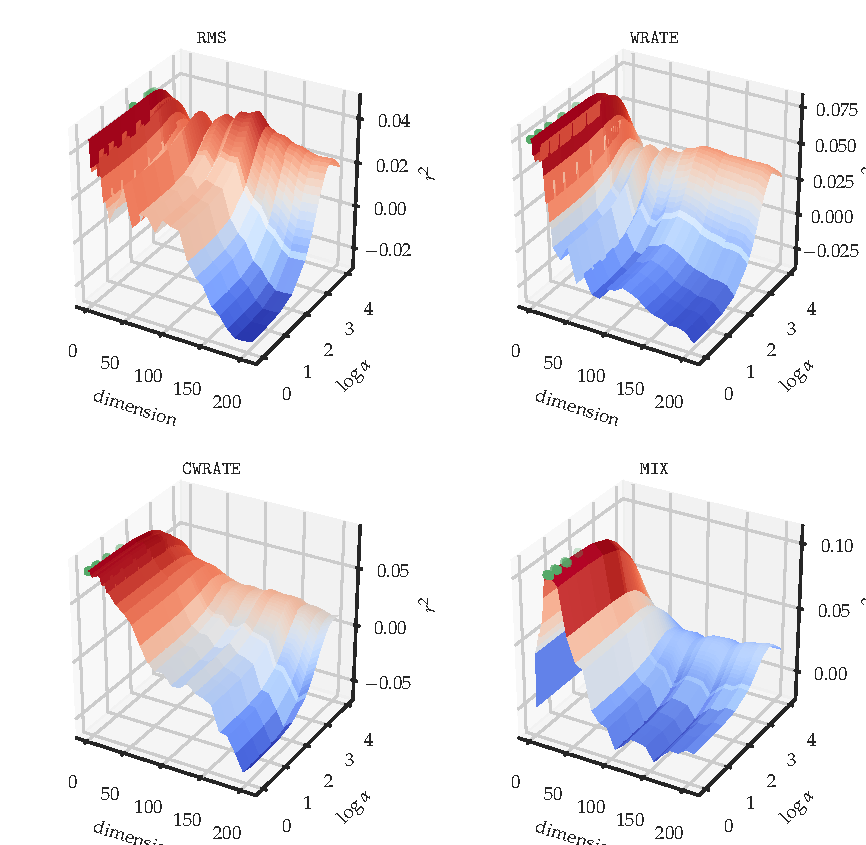
\includegraphics[scale=1]{Figures/TypicalVoxelDistributionS1R1.pdf}
    }
    \caption[Typical-Voxels' Response to \(\alpha\) and Dimension]{A selection of typical voxels found in \code{MIX} model regression results of subject 1 run 1. As shown by all four voxels, the regularization by large \(\alpha\) is beneficial only in higher feature dimensions. Our selection of \(\alpha\) contains a near-optimal value candidates for these voxels since the curve is all declining for the largest values. Green plots indicate the top 10 best configurations of the given voxel.} 
    \label{fig:TypicalVoxelDistributionS1R1}
\end{figure}

The optimal \code{r2}s of typical voxels are never attained at the upper bound of \(\alpha\) and dimension space. We plotted the heat-map for all voxels from the same run to verify if it is also the case at the whole-brain level (e.g. Figure \ref{fig:MIX_HeatmapAlphaDimS1R1}). We averaged 9 cross-validation run results to visualize subject-level best configuration distribution (Figure \ref{fig:MIX_HeatmapAlphaDimS1R0}). Histograms of best dimension and \(\alpha\) voxel-configuration of the averaged results are also plotted in Figure \ref{fig:MIX_CountPlotAlphaDimS1R0}. Plots for all runs and all subjects are available online\footnote{[TODO] add public url}. The analysis confirms that our parameter combination test range contains the near-optimal configuration for each voxel.

\begin{figure}
    \centering
    
    \makebox[.5\linewidth]{
            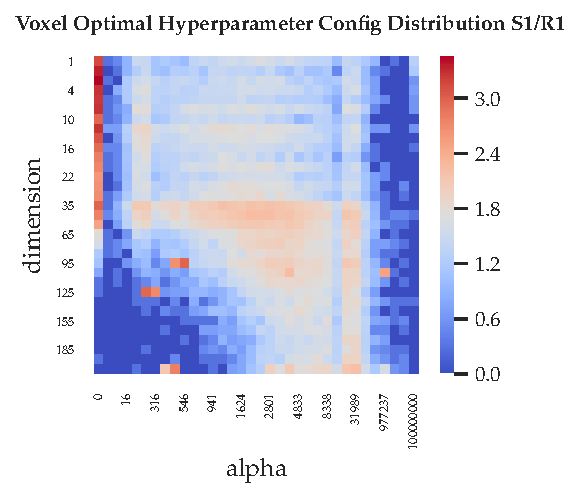
\includegraphics[scale=.8]{Figures/MIX_HeatmapAlphaDimS1R1.pdf}
            }
            \caption[Session Best Hyper-parameter Configuration Voxel-Count Heat-map]{[TODO fix title display] The scores are retrieved from \code{MIX} model regression for subject 1, fMRI run 1. Each cell represents an \(\alpha\) and dimension combination. The color indicates the logarithm of number of voxels having its global optimality with a given parameter set after having filtered out non-informative voxels (\code{r2} < 0). For small dimensions (< 35), small \(\alpha\)s (including 0) achieve the best performance. Starting from dimension 35, Ridge regularization with larger \(\alpha\)s is necessary.} 
            \label{fig:MIX_HeatmapAlphaDimS1R1}
   
\end{figure}

\begin{figure}
    \centering
    \makebox[\linewidth]{
    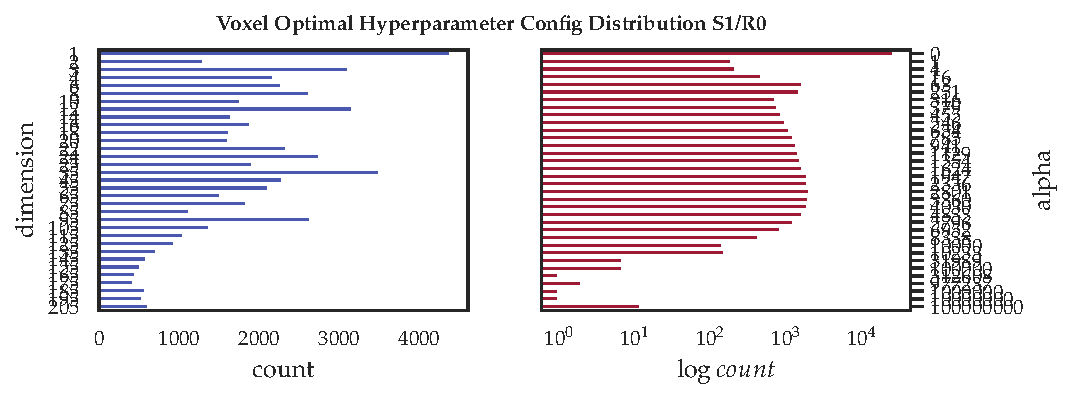
\includegraphics[scale=1]{Figures/MIX_CountPlotAlphaDimS1R0.pdf}
    }
    \caption[Best Hyper-parameter Configuration Voxel-Count Histograms]{[TODO, fix axis display] \textbf{Left panel}: Among informative voxels, a large portion of voxels are best modeled by \code{RMS} and \code{CWRATE} regressor classes. The addition of each semantic dimension from \code{MIX} improved a small proportion of voxel-models, marginal might be the contribution. \textbf{Right panel}: Most of the voxels are best modeled without Ridge regularization. The larger number obtained at \(\alpha=10000\) might indicate that larger alpha values might help better model a thousand voxels. A cumulation of voxel-count at the upper bound of the \(\alpha\) axis is noted: we performed post-hoc test for larger \(\alpha\) values than in the initial configuration, but the improvement of \code{r2} over the original score is marginal (\(<10^{-4}\)) for a sample of these voxels. A post-hoc analysis of larger \(\alpha\)s indicates a limited improvement of \code{r2}, thus for computational simplicity we kept the original Grid Search space of \(\alpha\).\label{fig:MIX_CountPlotAlphaDimS1R0}} 
    
\end{figure}

\subsubsection{\(\alpha\) Variability across Voxels}
[TODO: histogram animation with alpha evolution, ]

[TODO: discussion on overfit by dimension, despite regularization]




\subsection{Impact of \code{CWRATE}}
[TODO: Taking over SIM/ASN ? Visualize regression results without CWRATE]

\section{Embedding Model Brain Maps}
\subsection{\code{SIM} and \code{ASN} F-test}
\begin{table}
    \small
    \centering
    \begin{ThreePartTable}
        \begin{tabularx}{\textwidth}{l l p{1.5cm} *{3}{r} *{2}{P{1.2cm}}P{1.4cm}}
            \mc{6}{l}{\tabhead{\code{ASN} Best Improved Voxel Clusters}} \\
    \toprule
    \tabhead{Position} & \tabhead{BA} & \tabhead{Functional Label} & \tabhead{x} & \tabhead{y} & \tabhead{z} & \tabhead{\# Voxel} & \(\Delta\)\code{r2} \tabhead{Peak} & \(-\log_{10}\)\tabhead{ p-value} \\
    
    \toprule
    \mc{7}{l}{\tabhead{Top 4.7\%}}  &  > .0065 & >4.18   \\
    \midrule
    Temporal Mid L & 37 & Fusiform & -53 & -58 & -3 & 131 & .0121 & 4.35\\
    Frontal Inf Tri L & 46 & - & -46 & 37 & 11 & 68 & .0124 & 4.35 \\
    Occipital Mid L & 39 & - & -32 & -78 & 41 & 242 & .0125 & 4.35 \\
    Frontal Sup Medial L & 9 & - & -5 & 58 & 32 & 32 & .0092 & 4.35 \\
    Cingulum Mid L & 31 & - & -1 & -36 & 43 & 34 & .0105 & 4.35  \\
    Frontal Mid R & 8 & - & 28 & 15 & 46 & 63 & .0093 & 4.35  \\
    Angular R & 39 & - & 43 & -75 & 39 & 191 & .0114 & 4.35  \\
    Temporal Mid R & 21 & - & 46 & -32 & 0 & 182 & .0106 & 4.35 \\
    Frontal Inf Tri R & 46 & - & 50 & 35 & 8 & 56 & .0107  & 4.35\\
\bottomrule
    \end{tabularx}
    % \begin{tablenotes}
    % \footnotesize
    % \item[1] A cosine distance near 0 indicates a greater similarity.
% \end{tablenotes}  
\end{ThreePartTable}
\caption[\code{ASN} Voxel Improvement Clusters]{The Wilcoxon signed-rank test's p-value is thresholded at \(10^{-4.18}\) to make a clean cut is found in p-value histogram. Only 13 voxels reach a significance level of \(10^{-4.35}\) as is done with \code{ASN}. The voxel selection leads to top 4.7\% important voxel-model improvements. The largest \code{r2} boost is found in left MOccipital, followed by right mSTS, right Angular, left pFusiform bilateral iTriFrontal. Relatively smaller clusters are found in MCingulum L, L S Frontal BA9, R M Frontal BA8.  \label{tab:asnImprovementClusters}}
\end{table}
\begin{table}
    \small
    \centering
    \begin{ThreePartTable}
    \begin{tabularx}{\textwidth}{L l L *{3}{r} *{1}{R}}
    \mc{6}{l}{\tabhead{\code{CWRATE/SIM/SIG/ASN} F-test Significant Voxels}} \\
    \toprule
    \tabhead{Position} & \tabhead{BA} & \tabhead{Functional Label} & \tabhead{x} & \tabhead{y} & \tabhead{z} & \tabhead{\# Voxel in Region}\\
    \toprule
\code{CWRATE} \\
\midrule
    Fusiform L & 19 & - & -30.0 & -71.0 & -13.0 & 1 \\
Occipital Mid R & 19 & - & 46.0 & -77.0 & 3.0 & 1 \\
Cerebelum 8 R & 37 & Fusiform & 24.0 & -42.0 & -45.0 & 1 \\
Cerebelum 9 R & 37 & Fusiform & 8.0 & -52.0 & -35.0 & 1 \\
Lingual R & 18 & VisualAssoc & 8.0 & -90.0 & -7.0 & 1 \\
Precuneus R & 7 & - & 5.0 & -55.0 & 75.0 & 1 \\
Cingulum Post R & 30 & - & 2.0 & -33.0 & 12.0 & 1 \\
Occipital Sup L & 7 & - & -24.0 & -83.0 & 44.0 & 1 \\
Fusiform L & 18 & VisualAssoc & -24.0 & -83.0 & -16.0 & 1 \\
Lingual L & 18 & VisualAssoc & -24.0 & -90.0 & -16.0 & 1 \\
Cerebelum Crus2 R & 37 & Fusiform & 46.0 & -74.0 & -42.0 & 1 \\
Occipital Inf R & 37 & Fusiform & 52.0 & -68.0 & -13.0 & 1 \\
Occipital Inf L & 18 & VisualAssoc & -30.0 & -87.0 & -4.0 & 1 \\
Cerebelum Crus1 L & 18 & VisualAssoc & -33.0 & -87.0 & -26.0 & 1 \\
Cerebelum 8 L & 20 & - & -43.0 & -52.0 & -51.0 & 1 \\
Cerebelum Crus2 L & 37 & Fusiform & -43.0 & -64.0 & -38.0 & 1 \\
Cerebelum Crus2 L & 37 & Fusiform & -46.0 & -61.0 & -45.0 & 2.0 \\
Occipital Mid L & 19 & - & -49.0 & -74.0 & -0.0 & 1 \\
Temporal Pole Mid L & 38 & - & -52.0 & 11.0 & -35.0 & 1 \\
Cerebelum Crus2 L & 37 & Fusiform & -52.0 & -52.0 & -42.0 & 1 \\
Temporal Inf L & 37 & Fusiform & -55.0 & -45.0 & -23.0 & 1 \\
Cerebelum Crus1 L & 19 & - & -30.0 & -71.0 & -26.0 & 1 \\
Cerebelum 8 R & 37 & Fusiform & 36.0 & -55.0 & -51.0 & 1 \\
Temporal Pole Mid L & 38 & - & -55.0 & 11.0 & -32.0 & 1 \\
Rolandic Oper L & 6 & - & -62.0 & 2.0 & 9.0 & 1 \\

\toprule
\code{SIM} \\
\midrule
Temporal Mid L & 39 & - & -65.0 & -52.0 & 3.0 & 1 \\
Heschl L & 4 & PrimMotor & -65.0 & -11.0 & 9.0 & 1 \\
Temporal Mid L & 21 & - & -58.0 & -49.0 & 9.0 & 1 \\
Temporal Mid L & 39 & - & -55.0 & -55.0 & 3.0 &  1 \\
Temporal Sup R & 22 & - & 43.0 & -39.0 & 12.0 &  1 \\
\toprule
\code{SIG}\\
\midrule
Rolandic Oper R & 40 & - & 55.0 & -14.0 & 12.0 &  1 \\
Temporal Sup R & 22 & - & 58.0 & -30.0 & 3.0 &  1 \\
Temporal Sup R & 40 & - & 62.0 & -20.0 & 12.0 &  1 \\

\toprule
\code{ASN} \\
\midrule
Lingual R & 19 & - & 21.0 & -64.0 & -0.0 &  1 \\
Occipital Mid R & 18 & VisualAssoc & 33.0 & -80.0 & -0.0 &  1 \\

\bottomrule
    \end{tabularx}
    % \begin{tablenotes}
    % \footnotesize
    % \item[1] A cosine distance near 0 indicates a greater similarity.
% \end{tablenotes}  
\end{ThreePartTable}
\caption[\code{CWRATE/SIM/SIG/ASN} F-test Significant Voxels]{The most severe voxel score selection of \code{RMS} leads to left primary cortex (BA41) activation. Also well modeled voxels are distributed in more extensive areas of bilateral BA41 and right BA23 and BA10. With the addition of \code{CWRATE} features, voxel performances are systematically improved. With \code{CWRATE}, no other clusters appear in the thresholded voxel set. Left BA41 has a higher concentration of best modeled voxels, while right BA41 and cingulum mid R [TODO labels] degrade in voxel score ranking. Right BA10 also improves in ranking. \label{tab:Ftest}}
\end{table}

\subsection{\code{SIG} Nested Model and Contrast} 
\label{subsec:sig}
[TODO: replace SIM by SIG]

\begin{figure}
    \centering
    \makebox[\linewidth]{
    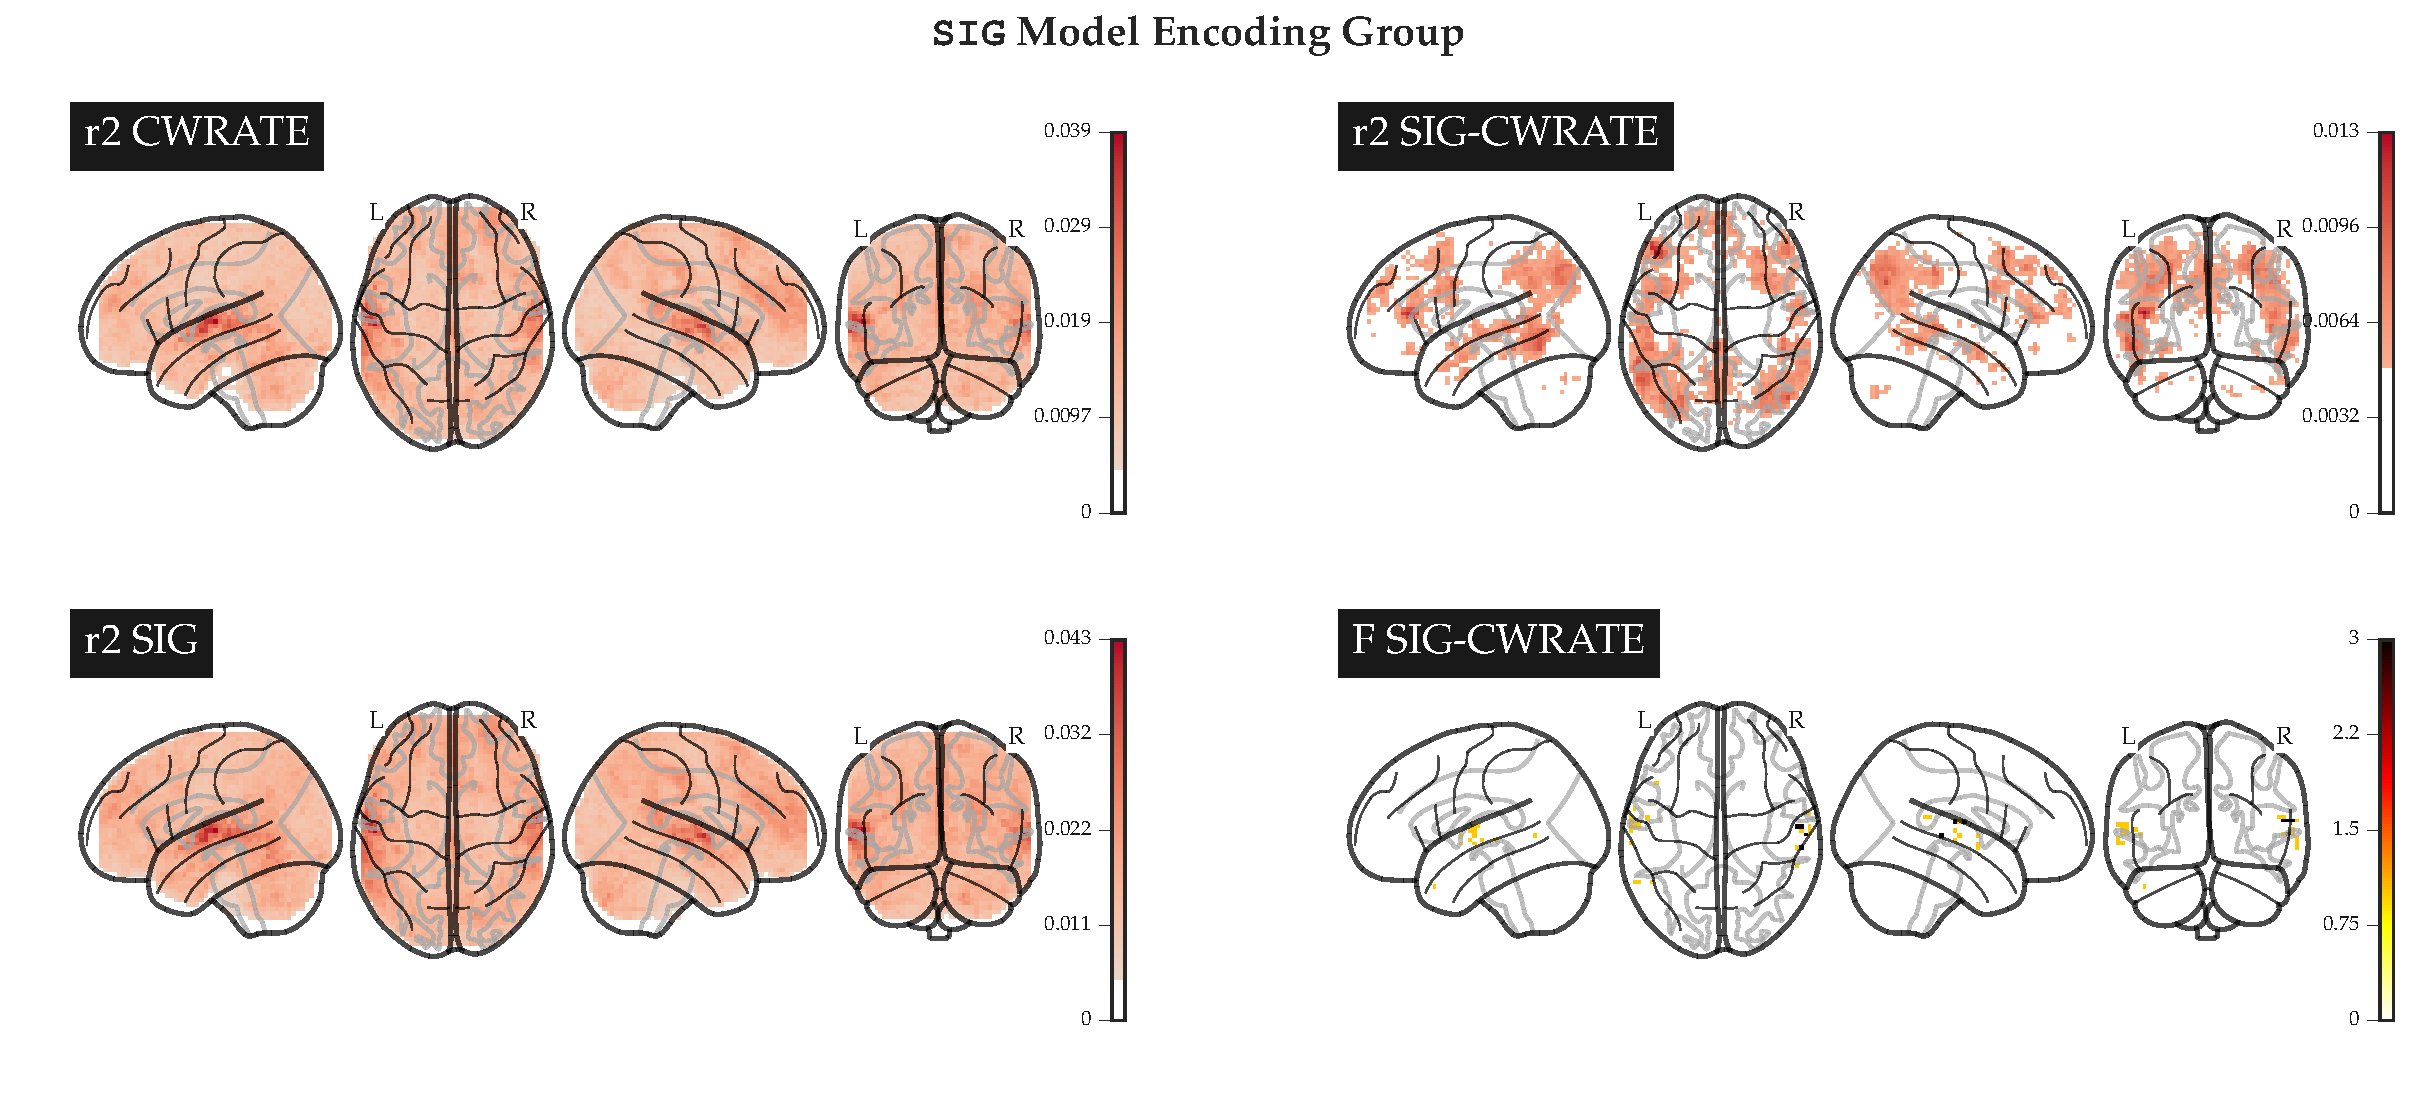
\includegraphics[width=.8\paperwidth]{Figures/SIG_ContrastMapG.pdf}
    }
    \caption[Encoding with \code{SIG} Features, Group]{[TODO]\textbf{Left panels}: The global activation pattern is unchanged with the feature addition. Best modeled zones are bilateral primary auditory cortices. \textbf{Right upper panel}  shows that \code{SIM} better models bilateral MTG, sup Parietal, Angular Gyrus (part of Wernicke's area), supramarginal gyrus and prefrontal areas (Table \ref{tab:simImprovementClusters}). F-test in \textbf{right lower panel} reports significant voxels in left pMTG BA21, 39, right pSTG BA22 and left Heschl BA4 (Table \ref{tab:Ftest}). Subject-wise results are available online at \url{http://bit.ly/micipsa_sim_wholebrain}.} 
    \label{fig:SIG_ContrastMapG}
\end{figure}


\begin{table}
    \small
    \centering
    \begin{ThreePartTable}
        \begin{tabularx}{\textwidth}{l l p{1.5cm} *{3}{r} *{2}{P{1.2cm}}P{1.4cm}}
            \mc{6}{l}{\tabhead{\code{SIG} Best Improved Voxel Clusters}} \\
    \toprule
    \tabhead{Position} & \tabhead{BA} & \tabhead{Functional Label} & \tabhead{x} & \tabhead{y} & \tabhead{z} & \tabhead{\# Voxel} & \(\Delta\)\code{r2} \tabhead{Peak} & \(-\log_{10}\)\tabhead{ p-value} \\
    \toprule
    \mc{7}{l}{\tabhead{Top .5\%}}  &  >.0079 & >4.35   \\
    \midrule
    Temporal Inf L & 37 & Fusiform & -56 & -56 & -12 & 85 & .0104 &4.35 \\
Frontal Inf Tri L & 46 & - & -46 & 35 & 12 & 35 & .0128 &4.35 \\
Parietal Sup L & 7 & - & -27 & -73 & 44 & 27 & .0093&4.35  \\
Angular R & 39 & - & 49 & -70 & 35 & 89 & .0105 &4.35 \\
Frontal Inf Tri R & 46 & - & 48 & 38 & 9 & 17 & .0088&4.35  \\
\bottomrule
    \end{tabularx}
    % \begin{tablenotes}
    % \footnotesize
    % \item[1] A cosine distance near 0 indicates a greater similarity.
% \end{tablenotes}  
\end{ThreePartTable}
\caption[\code{SIG} Voxel Improvement Clusters]{We thresholded Wilcoxon signed-rank test's significance at \(10^{-4.35}\) as a clean cut is found in p-value histogram, which leads to a selection of top .5\% important voxel-model improvements. The most significant and extensive cluster is found in left ITG, lateral Fusiform Gyrus, bilateral IFGtri (Broca's area), right angular gyrus (Wernicke's) and superior parietal gyrus. \label{tab:sigImprovementClusters}}
\end{table}
[SIG 209, No particularly different results are found. in PeaksSIG.ipynb]

[TODO, SIM->SIG]
We added with upon non semantic-embedding models \code{SIM} freatures to construct \similarity semantic models. While the whole-brain activation pattern stays globally unchanged (Figure \ref{fig:SIM_ContrastMapG} for group-wise average), in \code{SIM} voxel-models, left primary cortex are better ranked than in \code{BASE} model, while right mid cingulum models degrade (Table \ref{tab:rmsCluters}). \code{SIM} enlarges the performance superiority of left STG over right STG, indicating a left preference for textual semantic \similarity processing. The shrinkage of Mid Cingulum's proportion in top 1\% voxel models might imply that it has a limited participating in \similarity processing. The \code{r2} distribution analysis (Figure \ref{fig:SIM_ASN_Distribution} left) shows that in group-average \code{SIM} is informative for most of the voxel-models and none of voxels is overfitted by this addition. Table \ref{tab:simImprovementClusters} reports the most improved voxel clusters by \code{SIM} to be located in bilateral MTG, left Sup Parietal and right Angular Cortex (W=210, \(\Delta\)\code{r2}>0.0079, p-value<\(10^{-4.35}\) uncorrected). Left MTG improvements are more extensive and more important than right MTG. F-test results shows that \code{SIM} significantly improves isolated voxels (Table \ref{tab:Ftest}, p-value<0.05 voxel-wise multi-comparison corrected) in left pMTG BA21, 39, right pSTG BA22.


\subsubsection{With \code{SIG}}
\begin{figure}
    \centering
    \makebox[\linewidth]{
    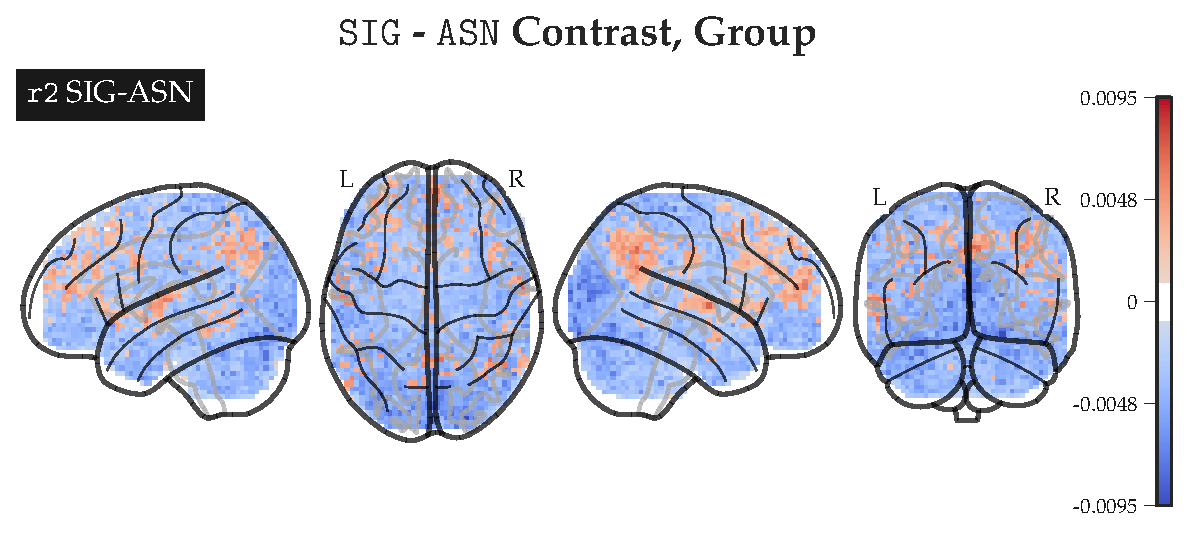
\includegraphics[width=.4\paperwidth]{Figures/EMB_SIG_ASN_r2_ContrastMapG.pdf}
    }
    \caption[\code{SIG}-\code{ASN} Contrast, Group]{[TODO]The differences of best voxel-model \code{r2}s are plotted. \code{SIM} preference is found in left BA10 SPFC, l aCC, l STS, l MPFC, r IParietal, r STG, MTG (Table \ref{tab:simasnContrastClusters_sim}) ... \code{ASN} preferences are found in bilateral BA18, RBA2-, l BA7 SParietal, R bA18, l BA37, l BA19, (visual association, fusimorm, primary visual, Parahip, and Thalamus). Subject-wise results are available online at \url{http://bit.ly/micipsa_sig_asn_contrast}} 
    \label{fig:EMB_SIG_ASN_ContrastMapG}
\end{figure}

\begin{table}
    \small
    \centering
    \begin{ThreePartTable}
        \begin{tabularx}{\textwidth}{l l p{1.6cm} *{3}{r} *{2}{P{.8cm}} P{1.3cm} P{.5cm}}


    \mc{6}{l}{\tabhead{\code{SIG-ASN} Voxel Contrast, Preference for \code{SIG}}} \\
    \toprule
    \tabhead{Position} & \tabhead{BA} & \tabhead{Functional Label} & \tabhead{x} & \tabhead{y} & \tabhead{z} & \tabhead{\# Voxel} & \(\Delta\)\code{r2} \tabhead{Peak} & \(-\log_{10}\)\tabhead{ p-value} & \tabhead{Cluster ID} \\
    \toprule

    Angular R & 39 & - & 39 & -55 & 28 & 8 &6.74&.0078& 1 \\
    Precuneus R & 31 & - & 8 & -55 & 41 & 13 &6.41&.0075& 2 \\
    Precuneus R & 23 & - & 8 & -55 & 25 & 4 &6.15&.0073& 3 \\
    \midrule
    Cingulum Ant L & 32 & - & -2 & 30 & 31 & 14 &5.94&.0072& 4 \\
    Cingulum Ant L & 32 & - & -11 & 34 & 22 &   &4.06&.0054& 4a \\
    Frontal Mid L & 10 & - & -36 & 49 & 15 & 3 &5.69&.0070& 5 \\
    Temporal Sup R & 41 & PrimAudi & 49 & -23 & 6 & 5 &5.45&.0068& 6 \\
    Precuneus L & 23 & - & -2 & -49 & 37 & 14 &5.38&.0067& 7 \\
    Cingulum Post L & 23 & - & -8 & -49 & 31 &   &3.81&.0052& 7a \\
    Caudate R & 48 & Caudate & 17 & 21 & 3 & 4 &5.38&.0067& 8 \\
    Frontal Sup Medial R & 10 & - & 5 & 56 & 15 & 4 &5.38&.0067& 9 \\
    Temporal Sup L & 41 & PrimAudi & -58 & -14 & 6 & 8 &5.30&.0066& 10 \\
    Precentral R & 8 & - & 39 & 8 & 44 & 2 &5.28&.0065& 11 \\
    Frontal Sup L & 10 & - & -27 & 59 & 25 & 2 &5.22&.0065& 12 \\
    Precentral L & 6 & - & -49 & 2 & 28 & 2 &5.03&.0063& 13 \\
    Temporal Sup L & 22 & - & -55 & -1 & -7 & 2 &4.98&.0062& 14 \\
    Temporal Inf L & 37 & Fusiform & -49 & -42 & -13 & 2 &4.77&.0060& 15 \\
    Temporal Sup R & 41 & PrimAuditory & 62 & -8 & 3 & 4 &4.70&.0060& 16 \\
    Cingulum Mid R & 23 & - & 5 & -20 & 34 & 6 &4.62&.0059& 17 \\
    Insula L & 47 & - & -36 & 18 & -13 & 2 &4.61&.0059& 18 \\
    Frontal Sup Medial R & 8 & - & 11 & 34 & 53 & 2 &4.57&.0059& 19 \\
    Angular R & 39 & - & 36 & -64 & 41 & 3 &4.57&.0059& 20 \\
    Caudate R & 48 & Caudate & 14 & 5 & 18 & 2 &4.46&.0058& 21 \\
    Parietal Sup L & 7 & - & -14 & -71 & 50 & 4 &4.46&.0058& 22 \\
    Temporal Mid L & 19 & - & -52 & -68 & 6 & 3 &4.29&.0056& 23 \\
    Frontal Inf Orb L & 47 & - & -46 & 21 & -7 & 2 &4.26&.0056& 24 \\
    Parietal Inf R & 40 & - & 46 & -42 & 41 & 2 &4.26&.0056& 25 \\
    Precentral R & 8 & - & 39 & 5 & 50 & 3 &4.24&.0056& 26 \\
    Cuneus L & 19 & - & -14 & -74 & 34 & 5 &4.05&.0054& 27 \\
    Frontal Sup Medial R & 10 & - & 5 & 62 & 12 & 3 &4.01&.0054& 28 \\
    Cingulum Mid L & 23 & - & -5 & -14 & 28 & 3 &4.00&.0054& 29 \\
    Cingulum Ant R & 32 & - & 5 & 43 & 3 & 3 &3.94&.0053& 30 \\
    Precuneus L & 7 & - & -14 & -68 & 31 & 2 &3.83&.0052& 31 \\
    Angular L & 39 & - & -46 & -64 & 47 & 2 &3.81&.0052& 32 \\
    Frontal Sup Medial R & 10 & - & 2 & 53 & 6 & 3 &3.79&.0052& 33 \\
    Frontal Sup Medial R & 10 & - & 8 & 59 & 22 & 5 &3.75&.0051& 34 \\
    Cingulum Mid L & 23 & - & -5 & -23 & 34 & 3 &3.74&.0051& 35 \\
    Precuneus L & 7 & - & -17 & -61 & 66 & 2 &3.73&.0051& 36 \\
    Frontal Sup Medial L & 9 & - & 2 & 56 & 34 & 2 &3.65&.0050& 37 \\
    Frontal Sup R & 8 & - & 21 & 37 & 53 & 2 &3.40&.0047& 38 \\
    Parietal Inf R & 40 & - & 43 & -45 & 44 & 2 &3.27&.0046& 39 \\
\bottomrule
    \end{tabularx}
    \begin{tablenotes}
            \footnotesize
            \item Voxel-wise Bonferroni corrected p=0.05 corresponds to uncorrected \(-\log_{10}\) p=6.04.
            % \item[*] Sub-peaks in one same cluster. 
        \end{tablenotes}  
    % \footnotesize
    % \item[] A cosine distance near 0 indicates a greater similarity.
% \end{tablenotes}  
\end{ThreePartTable}
\caption[\code{SIG-ASN} Voxel Contrast, \code{SIG}, Group]{The \code{SIG}-\code{ASN} contrast is computed by subtracting group-average voxel-wise \code{r2}. The significance is reported by two-tailed Wilcoxon signed-rank test before multi-comparison correction. The cluster is reported only if the average \code{r2} of \code{SIG} is higher than \code{ASN}. No cluster-size limit was applied when computing connected clusters. \code{SIG}'s model advantage over \code{ASN} is found in right angular gyrus and right medial parietal cortex. Left aSTG, right pSTG, left pITG, Frontal, limbic, parietal clusters are found significant before correction. \label{tab:sigasnContrastClusters_sig}}
\end{table}

\begin{table}
    \small
    \centering
    \begin{ThreePartTable}
    \begin{tabularx}{\textwidth}{l l p{1.6cm} *{3}{r} *{2}{P{1cm}} P{1.4cm} P{.5cm}}
        
    \mc{6}{l}{\tabhead{\code{SIG-ASN} Voxel Contrast, Preference for \code{ASN}}} \\
    \toprule
    \tabhead{Position} & \tabhead{BA} & \tabhead{Functional Label} & \tabhead{x} & \tabhead{y} & \tabhead{z} & \tabhead{\# Voxel} & \(\Delta\)\code{r2} \tabhead{Peak} & \(-\log_{10}\)\tabhead{ p-value} & \tabhead{Cluster ID} \\
    \toprule
Calcarine L & 17 & PrimVisual & 2 & -87 & 6 & 26 & - & 10.26 & 1 \\
Calcarine R & 17 & PrimVisual & 5 & -80 & 12 &   & .0095  & 8.30 & 1a \\
Cingulum Mid R & 32 & - & 17 & 5 & 37 & 2 & .0078 & 6.81  & 2 \\
Calcarine L & 18 & VisualAssoc & -2 & -99 & 12 & 2 & .0075& 6.27  & 3 \\
\midrule
Frontal Inf Orb R & 47 & - & 30 & 27 & -23 & 2 & .0065  & 5.25  & 4 \\
\bottomrule
    \end{tabularx}
    \begin{tablenotes}
        \footnotesize
        \item Voxel-wise Bonferroni corrected p=0.05 corresponds to uncorrected \(-\log_{10}\) p=6.04.
        % \item[*] Sub-peaks in one same cluster. 
    \end{tablenotes}  
    % \begin{tablenotes}
    % \footnotesize
    % \item[1] A cosine distance near 0 indicates a greater similarity.
% \end{tablenotes}  
\end{ThreePartTable}
\caption[\code{SIG-ASN} Voxel Contrast, \code{ASN}, Group]{The \code{SIG}-\code{ASN} contrast is computed by subtracting group-average voxel-wise \code{r2}. The significance is reported by two-tailed Wilcoxon signed-rank test before multi-comparison correction. The cluster is reported only if the average \code{r2} of \code{ASN} is higher than \code{SIG}. No cluster-size limit was applied when computing connected clusters. \label{tab:sigasnContrastClusters_asn}}
\end{table}



Section \ref{appsubsec:nonnestedcompres} suggests that first feature dimensions of \code{SIM} can be partially recovered by \code{ASN} model. Therefore, \code{ASN} might also be able to model voxels using less than 5 features from \code{SIM}, the result might thus lack low-level \code{SIM}/\code{ASN} contrast. As the first 4 dimensions of \code{SIM} encodes primarily POS information (Section \ref{appsubsec:projectorvisu}), we performed ad-hoc regressions on \code{SIM} space but uses only lemmas from a certain grammatical category to identify possible impacted regions. [TODO, supplementary]

The results found are consistent with the conjectures above: \code{ASN} scores are higher than \code{SIM} in average (Figure \ref{fig:SIM_ASN_Distribution} right), most of voxels respond better to \code{ASN} models (Figure \ref{fig:EMB_SIM_ASN_ContrastMapG}). As the Wilcoxon test shows (W=, \(\Delta\)\code{r2}>0.0068, p-value<0.05 voxel-wise multi-comparison corrected), only two significant clusters are found for \code{SIM} in ... (Table \ref{tab:simasnContrastClusters_sim}) and 17 are found for \code{ASN} (Table \ref{tab:simasnContrastClusters_asn}) in \dots.

The reported clusters for \code{SIM} are composed of 4 to 5 voxels. In our ROI analysis, ROIs larger than 26 voxels are used, thus none of the ROI revealed significance for \code{SIM}. As \code{ASN} has an overall dominance for almost all brain regions, small ROIs located in left m,p STG and large anatomical structures including IParietalLobe and Temporal Lobe all revealed their preference for \code{ASN} model. 

\begin{figure}
    \centering
    \makebox[\linewidth]{
    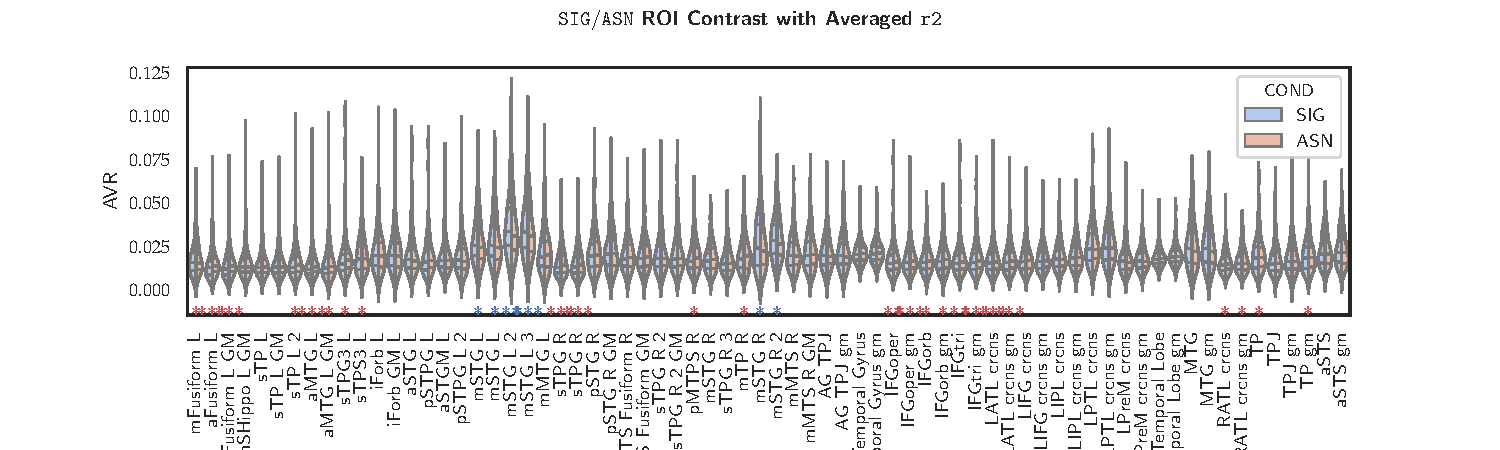
\includegraphics[width=\paperwidth]{Figures/SIG_ASN_ROI.pdf}
    }
    \caption[\code{SIG} \code{ASN} ROI Contrast, Group]{*: 0.05 uncorrected, ***: 0.05 ROI-wise multi-comparison corrected. Red color for \code{ASN}.\\ The average \code{r2} of voxels in a ROI is computed. We select only ROIs with scores>0.02 in either of \code{SIM} and \code{ASN} models. ROIs are of miminum size of 26 voxels (radius of 7 mm). None of the tested ROI reveals a significant mean difference in preference for \code{SIM}. ROIs in left (m,p)STG, l IParietalLobe, lTemporal Lobe respond better to \code{ASN} model.} 
    \label{fig:SIG_ASN_ROI}
\end{figure}

% \subsection{\code{MIX} Nested Model and Contrast}
% [TODO: contrast MIX with SIM, ASN, SIG]

\section{On Behavioral Control}

The correlation between cross-validation session-wise model performances consistently correlates with participants' comprehension question scores in the end of each validation fMRI recording.

\begin{table}
    \centering
    \begin{tabularx}{\textwidth}{L  *{8}{l}}
    \mc{8}{l}{\tabhead{Correlation of Model Performance with Comprehension Question Scores}} \\
    \toprule
    &\mc{2}{c}{\code{SIM}} & \mc{2}{c}{\code{SIG}}& \mc{2}{c}{\code{ASN}} & \mc{2}{c}{\code{MIX}} \\
    \cmidrule{2-3}\cmidrule{4-5}\cmidrule{6-7}\cmidrule{8-9}
    & max & mean & max & mean & max & mean & max & mean \\
    \toprule
    Pearson's r & -.15 & -.17 & -.16 & -.18 & -.09 & -.12 & -.11 & -.14 \\
    p & .0466 & .0221 & .0262 & .0173 & .1329 & .0593 & .4296 & .3893\\
\bottomrule
    
    \end{tabularx}
    \caption[Model Performance and Behavioral Question Score Correlation]{}
    \label{tab:behavioral}
    \end{table}

